%\setmainlanguage{german}
\section{Auswertung}
\subsection{Entladevorgang}
Um die Zeitkonstante \tau zu bestimmen, wird der Entladevorgang des Kondensators anhand der Spannung gemessen.
Darüber hinaus werden die Messwerte aus Tabelle \ref{tab:a} in einem halblogarithmischen Diagramm aufgetragen und durch lineare Regression mit folgender Formel ausgewertet.
\begin{equation}
    y = m \cdot x +b
\end{equation}
Dabei wird die Zeit gegen den natürlichen Logarithmus der gemessenen Spannung in Diagramm 1 aufgetragen
Es ergibt sich aus dem Logarithmieren von (6), dass die Steigung $m$ der Ausgleichsgeraden dem Inversen der Zeitkonstante $\tau$ entspricht.
Dabei ergibt sich dann Folgendes.
\begin{equation}
    \ln(U(t)) = \ln(U_0 e^{\frac{-t}{RC}}) = \ln(U_0) - \frac{t}{RC}
\end{equation}
Somit folgt für die lineare Regression und die Zeitkonstante.
\begin{align}
    m  =  \SI{-710.610 \pm 7.038}{\frac{1}{s}} \notag
\end{align}
\begin{equation}
    b = 4.693 \notag
\end{equation}
Und letztendlich lässt sich die Zeitkonstante mit der Gaußschen Fehlerfortpflanzung aus (11) und (12) auf folgenden Wert bestimmen.
\begin{equation}
    \tau = RC = - \frac{1}{m} = \SI{1,407 \pm 0,014}{ms} \notag
\end{equation}
Die folgende Gleichung beschreibt die Gaußsche Fehlerfortpflanzung.
\begin{equation}
    \increment \tau = \sqrt{\left (\frac{\partial \tau}{\partial m} * \sigma_{m} \right )^2}	\notag
\end{equation}

\begin{table} [H]
	\centering
	\caption{Entladevorgang}
	\label{tab:a}
	\sisetup{table-format=4.2}
	\begin{tabular}{S[table-format=4.2] S S S S [table-format=3.2]}
		\toprule
		{$\increment t / \text{\mu s}$} & {$U / \text{V}$} \\
		\midrule
		0 & 108,8 \\
		20 & 107,2 \\
		40 & 105,6\\
		60 & 104,8 \\
		80 & 103,2 \\
		100 & 101,6 \\
		120 & 100,0 \\
		140 & 98,4 \\
		160 & 97,6 \\
		180 & 96,0 \\
		200 & 94,4 \\
		250 & 91,2 \\
		300 & 88,0 \\
		350 & 84,8 \\
		400 & 82,4 \\
		450 & 80,0 \\
		500 & 76,0 \\
		600 & 71,2 \\
		700 & 66,4 \\
		800 & 61,6 \\
		900 & 57,6 \\
		1000 & 53,6 \\
		1100 & 50,4 \\
		1200 & 47,2 \\
		1500 & 38,4 \\
		1800 & 30,4 \\
		2100 & 24,8 \\
		2400 & 19,2 \\
		7000 & 0 \\
		\bottomrule 
	\end{tabular}
\end{table}
\begin{figure}[h]
    \centering
    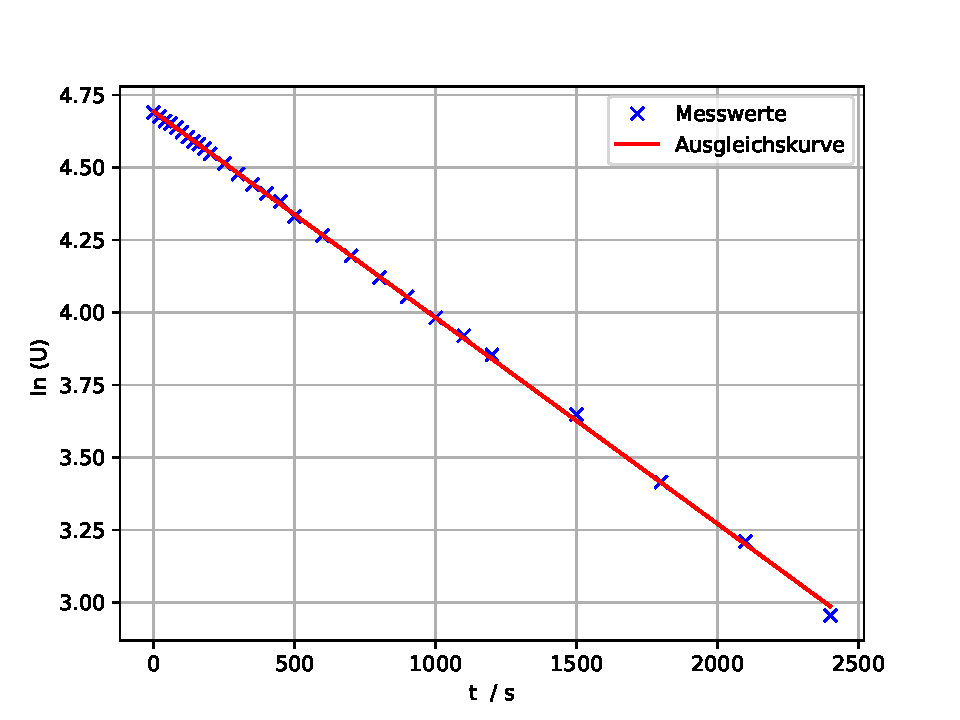
\includegraphics{Entladekurve.pdf}
    \caption{Entladekurve des Kondensators}
    \label{fig:a}
\end{figure}

\subsection{Frequenzabhängigkeit der Amplitude}

Hierbei werden die in der Tabelle \ref{tab:b} eingetragengen Werte in einem halblogarithmischen Diagramm aufgetragen.
Aus (10) folgt mithilfe nichtlinearer Regression folgender Wert für die Zeitkonstante.
\begin{equation}
	\tau = RC = \SI{1,42 \pm 1,217}{10^{-7}ms} \notag
\end{equation}

Das dazugehörige Diagramm 2 beschreibt die dazugehörige Ausgleichskurve.

\begin{table} [H]
	\centering
	\caption{Frequenzabhängigkeit der Amplitude}
	\label{tab:b}
	\sisetup{table-format=4.2}
	\begin{tabular}{S[table-format=5.2] S S S S [table-format=3.2]}
		\toprule
		{$f / \text{Hz}$} & {$U_0 / \text{V}$} \\
		\midrule
		10 & 50,00 \\
		20 & 50,00 \\
		40 & 47,60 \\
		60 & 44,40 \\
		80 & 41,20 \\
		100 & 37,60 \\
		200 & 25,20 \\
		300 & 17,20 \\
		400 & 13,70 \\
		500 & 11,10 \\
		750 & 7,50 \\
		1000 & 5,50 \\
		2000 & 2,84 \\
		3000 & 1,88 \\
		4000 & 1,94 \\
		5000 & 1,16 \\
		10000 & 0,58 \\
		20000 & 0,30 \\
		30000 & 0,22 \\
		40000 & 0,16 \\
		50000 & 0,12 \\
		\bottomrule 
	\end{tabular}
\end{table}
\begin{figure}[h]
    \centering
    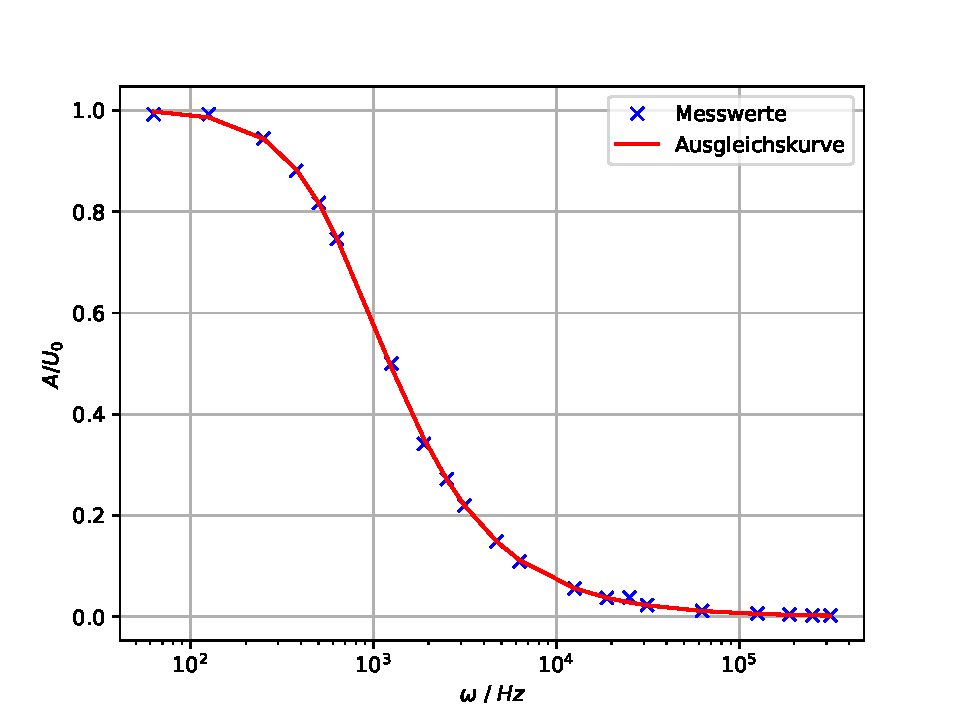
\includegraphics{Plot2.pdf}
    \caption{Frequenzabhängige Spannung am Kondensator}
    \label{fig:b}
\end{figure}

\subsection{Phasenverschiebung}
Die Zeitkonstante kann auch durch die Messung der Phasenverschiebung bestimmt werden.
Hierbei wurde die Phasenverschiebung mit folgender Gleichung bestimmt.
\begin{equation}
	\varphi = \frac{a}{b} \cdot 2\pi
\end{equation}
Dabei ist $a$ der Abstand der Nulldurchgänge und b die Periodendauer der beiden Schwinungen, die identisch ist.
Diese Werte wurden für verschiedene Frequenzen bestimmt und in Tabelle \ref{tab:c} aufgetragen.

Aus (8) und (9) kann dann der Quotient der Amplitude und der Ausgangsspannung folgendermaßen beschrieben werden.
\begin{equation}
	\frac{A}{U_0} = -\frac{sin(\varphi)}{\omega RC}
\end{equation}
Eine nichtlineare Ausgleichsrechnung nach (15) liefert dann folgenden Wert.
\begin{equation}
	\tau = RC = \SI{1,58 \pm 4,450 }{10^{-4}{ms}}
\end{equation}

\begin{table} [H]
	\centering
	\caption{Phasenverschiebung}
	\label{tab:c}
	\sisetup{table-format=4.2}
	\begin{tabular}{S[table-format=4.2] S S S S [table-format=3.2]}
		\toprule
		{$f / \text{Hz}$} & {$\varphi / rad$} \\
		\midrule
		10 & 0,73 \\
		20 & 0,55 \\
		30 & 0,49 \\
		40 & 0,60 \\
		60 & 0,68 \\
		80 & 0,68 \\
		100 & 0,75 \\
		200 & 1,13 \\
		400 & 1,41 \\
		600 & 1,43 \\
		800 & 1,46 \\
		1000 & 1,51 \\
		2000 & 1,63 \\
		\bottomrule 
	\end{tabular}
\end{table}

\begin{figure}[h]
    \centering
    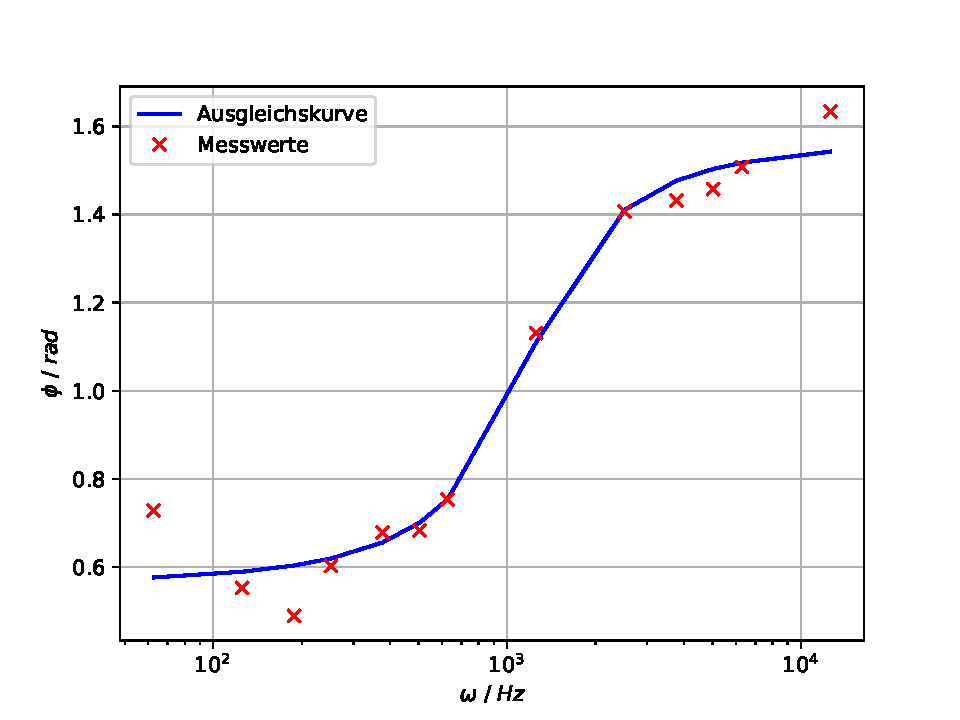
\includegraphics{Phasenverschiebung.pdf}
    \caption{Phasenverschiebung am Verhältnis der Amplitude}
    \label{fig:c}
\end{figure}
\begin{figure}[h]
    \centering
    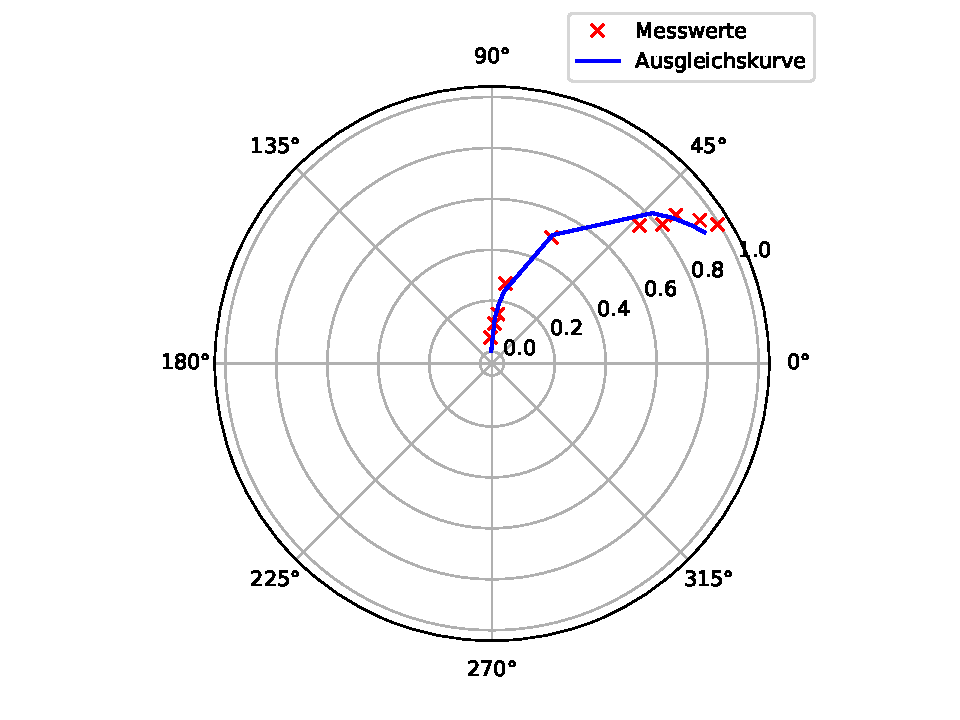
\includegraphics{Polar.pdf}
    \caption{Polardiagramm mit Relativamplitude $\frac{A}{U_0}$ gegen die Phasenverschiebung $\varphi$}
    \label{fig:d}
\end{figure}

\subsection{Integrität}
Der letzte Versuchsteil beschäftigt sich mit der Integrationsfähigkeit eines RC-Kreises.
Dabei werden drei verschiedene Eingangsspannnungen verwendet.
Nach (11) wurden eine Rechtecks-, Dreiecks- und Sinusspannung inegriert und experimentell überprüft.
Zunächst die Rechtecksspannung.
\begin{equation}
	f_\text{Rechteck}(t)=\left\{\begin{array}{ll} A & 0 \leq t \leq d \\
		-A & d \leq t \leq 2d\end{array}\right.
\end{equation}

Integriert man diese Funktion so ergibt sich Folgendes.
\begin{equation}
		F_\text{Rechteck}(t)=\left\{\begin{array}{ll} A \cdot t & 0 \leq t \leq d \\
			-A \cdot t & d \leq t \leq 2d\end{array}\right.
\end{equation}
Die Stammfunktion würde also theoretisch einer Dreiecksspannung entsprechen.
Die nächste untersuchte Funktion ist die Dreiecksspannung.
\begin{equation}
		f_\text{Dreieck}(t)=\left\{\begin{array}{ll} A \cdot t & 0 \leq t \leq d \\
			-A \cdot t & d \leq t \leq 2d\end{array}\right.
\end{equation}
\begin{equation}
		F_\text{Dreieck}(t)=\left\{\begin{array}{ll} \frac{A}{2} \cdot t^2 & 0 \leq t \leq d \\
			-\frac{A}{2} \cdot t^2 & d \leq t \leq 2d\end{array}\right.
\end{equation}
Die integrierte Funktion würde einer Sinusspannung entsprechen.
Zuletzt wird eine Sinusspannung untersucht.
\begin{equation}
	f_\text{Sinus} = A \cdot sin(t)
\end{equation}
\begin{equation}
	F_\text{Sinus} = -A \cdot cos(t)
\end{equation}

\begin{figure}[h]
    \centering
    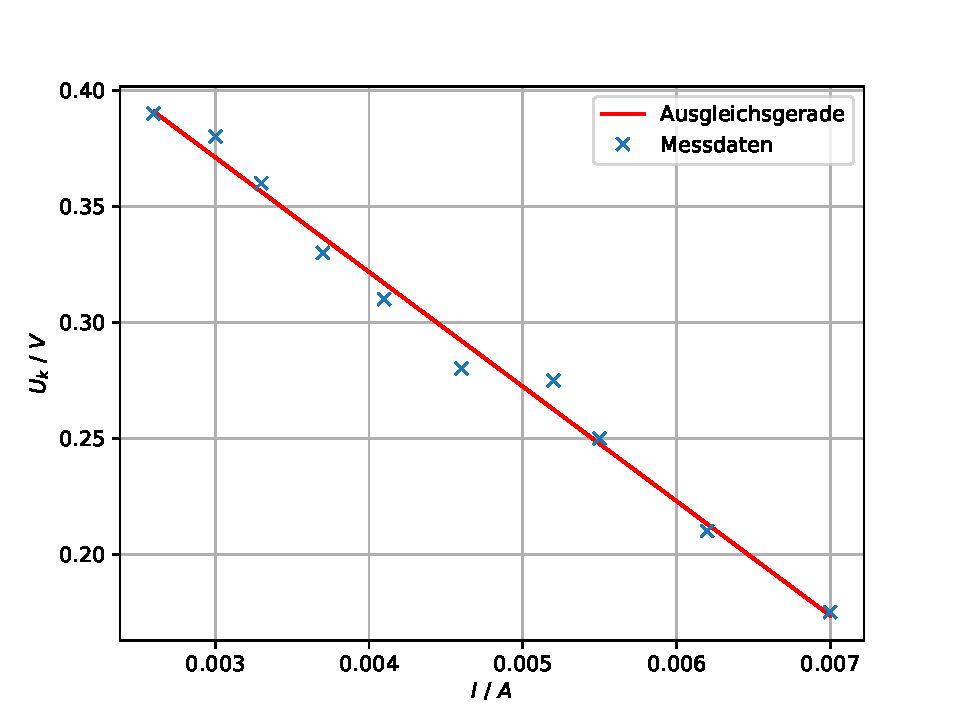
\includegraphics[width=6.5cm]{Rechteck.pdf}
     \caption{Rechteck- und integrierte Rechteckspannung}
    \label{fig:e}
\end{figure}
\begin{figure}[h]
    \centering
    \includegraphics[width=6.5cm]{Dreieck.pdf}
     \caption{Dreieck- und integrierte Dreieckspannung}
    \label{fig:f}
\end{figure}
\begin{figure}[h]
    \centering
    \includegraphics[width=6.5cm]{Sinus.pdf}
     \caption{Sinus- und integrierte Sinusspannung}
    \label{fig:g}
\end{figure}